% Background - extensão universitária no Brasil, curricularização da extensão, soluções/ferramentas de apoio à extensão, leis federais, resoluções unipampa, implantação da extensão, tipos de extensão, perfis de pessoas envolvidas na extensão, programas e projetos de extensão na unipampa
% Unipampa Cidadã
%=====================================
\chapter{Background}\label{background}
%=====================================

In this chapter, information that complement the objective of the study are discussed, helping to understand the policies and resolutions involved. In \Cref{sec:bac-outreach-brazil} the national outreach activity policy will be presented, which is valid for all \acp{HEI} in Brazil. It applies for each \ac{OA} regarding its relation to the academic and external community. Soon after in \Cref{sec:bac-higher-ed} and \Cref{sec:bac-unipampa} the vision of how both the \acp{HECI} as a whole and \acl{UNIPAMPA}, respectively, adapted to receive these new rules is described. Afterwards, in \Cref{sec:bac-programs-projects} the differences between outreach programs and projects will be presented, followed by how new proposals are handled in \Cref{sec:bac-proposals}. Then, a more detailed explanation about the ``\ac{UNIPAMPA} Cidadã'' project is described in \Cref{sec:bac-cidada}. \Cref{sec:bac-tools} showcases current available tools and solutions in the market which are related to the study goal product. Finally in \Cref{sec:bac-summary} a general summary of the chapter is presented.

\section{Outreach activities in Brazil}\label{sec:bac-outreach-brazil}

It is clear that participating in outreach activities has many benefits for the students who decide to take part in it \cite{sellou2011many}. Besides promoting individual growth, the activities can also serve as a bridge connecting students and professors even more. In order to preserve them and encourage younger students to participate in them, the \acl{FORPROEX} (\ac{FORPROEX}), updated the old version of the National Outreach Policy document, published in 1999, with current situations and challenges encountered in recent years. In the new version of the document, \cite{politicaNacional}, some of its objectives are the following:

\begin{itemize}
  \item Achieve the recognition of university outreach activities as an essential tool for the public university.
  \item Ensure that the outreach activity is the solution to any type of social problem faced by the country.
  \item Defend the funding of outreach programs and projects so that they can continue to function.
  \item Promote environmental and sustainable awareness in outreach projects in Brazil.
  \item Promote solidarity both nationally and internationally, covering the area of impact of outreach actions.
\end{itemize}

As a reference for directing and assisting \acp{HECI} to create their outreach policies, \cite{referenciaisPolitica} also highlights the importance of integrating outreach activities with research and teaching, along with discussions of a social nature and the effects of the results on society. The document proposes nine outreach activity types, which are as follows:

\begin{inparaenum}[(1)]
  \item Programs, Projects and Activities for the socialization of knowledge;
  \item Outreach Courses;
  \item Participation in Councils, Academic Events open to the external community: Congresses, Symposia, Seminars, Colloquiums, Course Weeks and related activities;
  \item Promotions of Art, Culture, Sport and Leisure with the involvement of the external community;
  \item Provision of Services, Consultancy and Advisory Services, Technological Extension, Mandatory Internships;
  \item School Clinics;
  \item Curricular Professional Practices;
  \item Course subjects that include practices with external communities;
  \item Research Projects, Course Completion Works,
  Monographs, Dissertations and Theses with methodologies and practices of social intervention with external communities.
\end{inparaenum}

\subsection{\acl{OA} curricularization in Higher Education}\label{sec:bac-higher-ed}

In order to implement what was mentioned above in the \ac{HECI}, the Brazilian Ministry of Education created the Resolution No. 7, of December 18, 2018, which establishes guidelines, principles, foundations and procedures for \acp{OA} in higher education. As such, it was regulated that \acp{OA} will be made available in the form of curricular components for the offered courses \cite{ministerioSuperiorExtensao}.

The document also determines that the outreach activities must comprise at least 10\% (ten percent) of the total student curricular workload of undergraduate courses, and they must also be part of the curriculum of the courses \cite{ministerioSuperiorExtensao}. Another important discussed topic is about the self-assessment of \acp{OA}. The main reason for this is the constant improvement of the activity with teaching, research, student training, teacher qualification, the relationship with society, the participation of partners and other institutional academic dimensions.. This evaluation must include the following:

\begin{inparaenum}[(a)]
  \item How many curricular credits the activity can give;
  \item How it contributes to the Institutional Development Plan and the Pedagogical Projects for the Courses;
  \item The demonstration of the results achieved in relation to the participating public.
\end{inparaenum}

Each \ac{OA} must also contain the planning of its internal activities, the strategies for self-assessment, proposal, development and conclusion. These must be duly recorded and analyzed in order to organize the activity work plans.

As a final note, the \textcite{ministerioSuperiorExtensao} says that the \acp{HEI} will have at most 3 (three) years, counting by the date the document was published, to implement what is being proposed.

\subsection{\acl{OA} curricularization in \acl{UNIPAMPA}}\label{sec:bac-unipampa}

In relation to \ac{UNIPAMPA}, as with other \ac{HECI}, it must create a resolution aimed at standardizing outreach activities in general, presenting what they are, their target audience and their objectives. And thus was born the CONSUNI/UNIPAMPA Resolution No. 332 of 2021, which determines the types of outreach activities, already mentioned earlier in the study, their managing bodies, executing team, possible related processes, and rules such as the minimum duration of 8 (eight) hours \cite{Resolucao-332:2021}.

As \ac{UNIPAMPA} highlights in the Resolution No. 317 of 2021, the main objectives in the insertion of outreach activities in undergraduate courses are the following \textcite{res317}:
\begin{inparaenum}[(i)]
  \item Help students develop their critical, civic, interdisciplinary and responsible education;
  \item Improve teaching in undergraduate courses as a whole and strengthen the inseparability between teaching, research and outreach;
  \item Strengthen \ac{UNIPAMPA}'s social commitment;
  \item Stimulate constructive discussions in all sectors of \ac{UNIPAMPA};
  \item Promote actions that strengthen \ac{UNIPAMPA}'s ethical principles and social commitment in all areas;
  \item Encourage the academic community to be more present in human, academic, social, cultural and economic development.
\end{inparaenum}

\subsection{Outreach Programs and Projects}\label{sec:bac-programs-projects}

According to \textcite{referenciaisPolitica}, Outreach Program and Projects are activities regulated by the institution that articulates events involving teaching and research, always involving the external community. With them students can make decisions directly about the community in which they live, contributing to their evolution and progress.

\textcite{Viero} describes the difference between programs and projects as follows: A project is a set of educative actions of social, cultural or technological nature, with a specific objective and determined deadline. An outreach program is a set of projects, which is preferably multidisciplinary and integrated with research and teaching activities.

A good example of an outreach program is \textcite{JEDI}, which, as mentioned earlier in \Cref{introduction}, aims to solve local problems using technology and involvement with the community. In the first cycle of the program four outreach projects were proposed, each with its own objectives, methodologies and activities:
\begin{inparaenum}[(i)]
  \item Padawan Academy;
  \item Jedi Apprentice;
  \item Jedi Problem-Solving;
  \item Jedi Mind.
\end{inparaenum}

\subsection{Workflow for \acl{OA} Proposals}\label{sec:bac-proposals}

As briefly mentioned in \Cref{sec:bac-unipampa}, \textcite{Resolucao-332:2021} defines a few requirements which must be met before creating new outreach projects or programs. The \acl{UNIPAMPA} created a few workflow visualizations in order to better understand how the process works.

% pedir imagens svg ao igor

In \Cref{fig:outreach-projects-registration}, the registration flow of a new outreach project is presented. It is possible to see that the proposal goes through several steps of corrections and evaluations, being sent to several actors throughout the whole process. Finally, the \acl{PROEXT} is the responsible entity to request final changes or approve the project, granting a new registration number.

\begin{figure}[!htb]
  \caption{Outreach Projects Registration}\label{fig:outreach-projects-registration}
  \begin{center}
    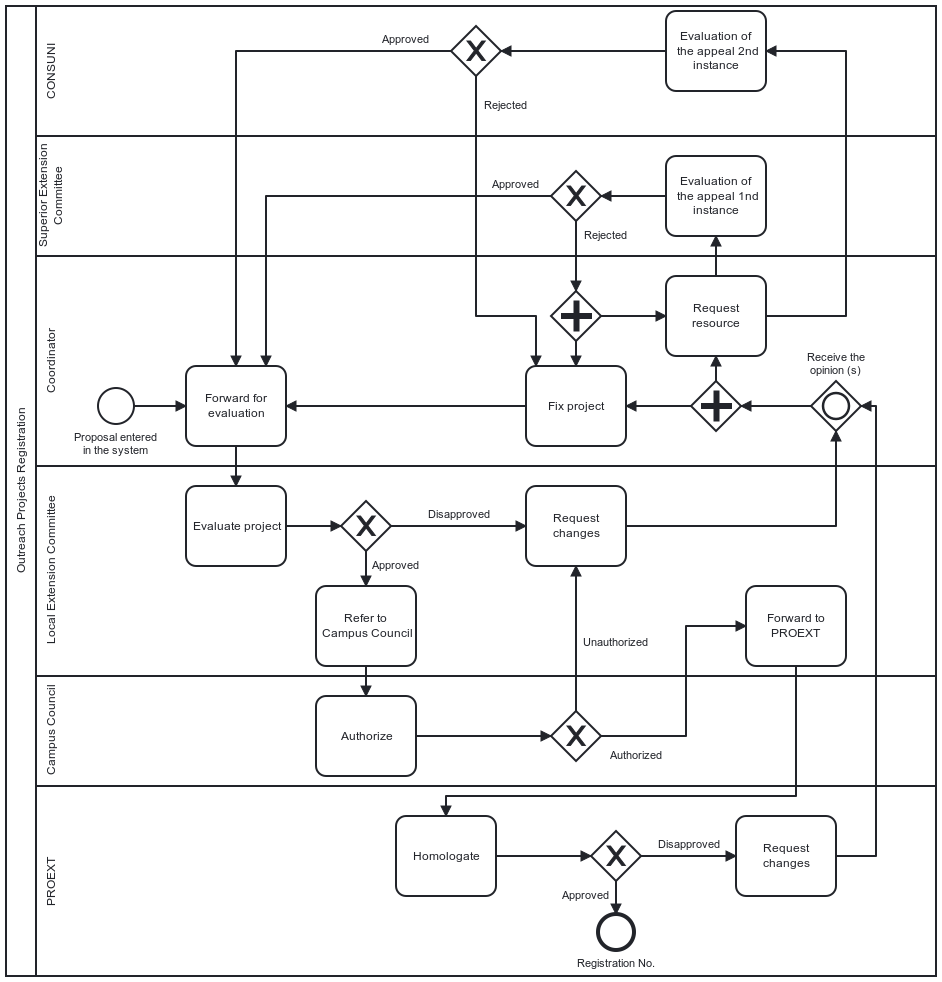
\includegraphics[width=16cm]{img/3-registroDeProjetosDeExtensaoV3.png}
  \end{center}
  \fonte{Adapted from \cite{siteProcessos}.}
\end{figure}

In addition, \Cref{fig:issuance-certificates} presents the steps related to the approval and generation of certificates. Firstly, the proponent of the activity must have the presence list and spreadsheet with information for the generation of certificates. Afterwards, a final report is created and inserted into the \ac{SIPPEE} system. This report is then evaluated and approved, returning to \ac{PROEXT}, who, with the information spreadsheet, sends this data to the \ac{SGCE} system, finally receiving the certificates and sending them to participants' emails.

\begin{figure}[htb]
  \caption{Issuance of Certificates}\label{fig:issuance-certificates}
  \begin{center}
    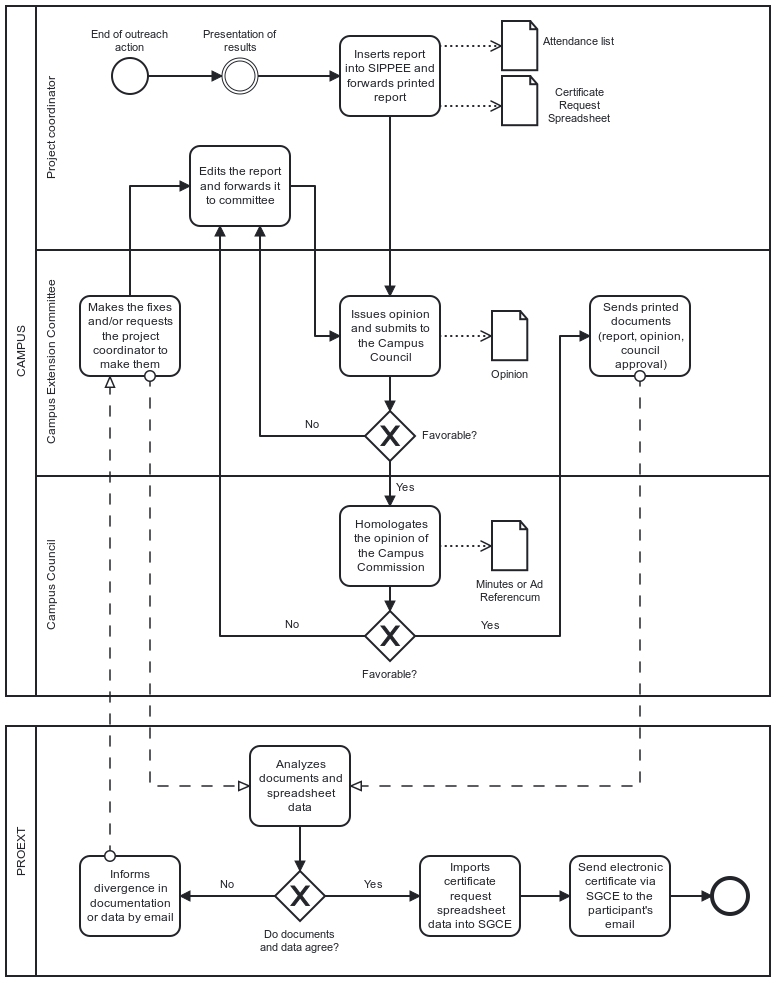
\includegraphics[width=16cm]{img/3-emissaoDeCertificados.png}
  \end{center}
  \fonte{Adapted from \cite{siteProcessos}.}
\end{figure}

\subsection{UNIPAMPA Cidadã}\label{sec:bac-cidada}

The \acl{UNIPAMPA}, through Normative Instruction No. 18 \cite{unipampacidada}, making use of Resolution No. 317, \cite{res317}, establishes the outreach project called ``Unipampa Cidadã'' (Unipampa Citizen). It must be offered by all courses, consisting of citizenship and solidarity activities and with the objective of forming graduates aware of their social responsibility, stimulating and increasing integration with the local community.

After the implementation of the project in the institution's courses, the subject offered for the project must be at least 60 and at most 120 hours, and is required to be taken by all students. The community actions must be carried out in public institutions, \aclp{NGO} and organizations or organized civil society associations. The course outreach supervisor is the one in charge of making the evaluation, planning, monitoring and validation of the project, as well as defining the beginning of the activities.

The project also describes in Normative Instruction No. 18 a form that must be filled when activities are finished. This way, the student will be able to reflect on the impact of the project under his vision, pointing out what he learned during the project's execution. The supervisor can make observations on the student and indicate if he has been approved or not.

\section{Similar Tools}\label{sec:bac-tools}

As \Cref{greyliterature} will later present in more detail the systematic review performed in the grey literature, a research has been done to collect tools related to outreach activities which are available currently in the market. With the results it was possible to list features, details and common points among the tools.

A lot of interesting and different results were found and analyzed, generating artifacts and describing all the cool and unique features each of them had. During the review, the tool that returned the most results and was always present in the search results, was \ac{SIGAA}. However, its scope reaches way beyond just managing outreach activities. It contains features for most processes present in an institution. Another that presented interesting results was \ac{CAEX}, which had several unique features. Overall, it was possible to retrieve ideas of great importance and find inspiration to build a new related product.

\section{Chapter Summary}\label{sec:bac-summary}

This chapter presented guidelines of several resolutions and normatives related to outreach, both in the country as a whole, and in the \acl{UNIPAMPA}. It was also discussed about the similarities and differences between the outreach programs and projects, presenting the most relevant processes involved in their lifecycle. As a recent example of an outreach program, ``Unipampa Cidadã'' (Unipampa Citizen) had part of its objectives and guidelines presented. Finally, it was also discussed a little about the systematic review in the grey literature and the similar tools found. The next chapter aims to discuss more about criteria, methodology, results, research questions, and other relevant information related to the grey literature systematic review.